This section shows the results of the experiment explained. First, the results of training the source models  will be shown, followed by the results from the transfer
learning experiments.
In fact, in the original model, before the improving, has accuracy of 98.50\%, a precision of 99.39\%, a recall of 98.79\%, an F1 score of 99.09\%, and a training time of 1 min 10 s, while the model after improving to efficient db gave the precision score 85 for class 0 (edible) , and 85\% of actually edible,  precision score was 88\% for the class 1 (poisonous mushrooms)  and 88\% of actually poisonous.
The recall score of 86\% for class 0 (edible mushrooms), and the recall score of 87\% for class 1 (poisonous mushrooms). It's cleasr that the model correctly identified 86\% edible to edible. The model correctly identified 87\% poisonous to poisonous.

The reason for this could be that the dataset were used in our experiment were more diverse. With hundreds of different-looking mushrooms, it may have been difficult for our model to remember those different patterns. Some types also have very few images, such as 12 to 15 images. With only 12 to 15 images to learn the pattern, it is difficult for the machine. 
in addition, adding more images in each type folder is a time consuming work and maybe in the next research this strategy can be implemented. But due to time constraints and also due to limitations in GPU power, we decided not to enlarge the images.



\subsection{Classification}
\centering
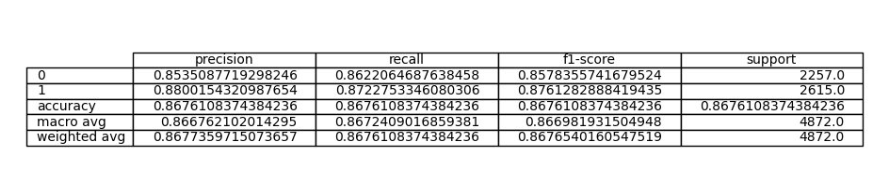
\includegraphics[width=.5\textwidth]{figures/classification.PNG}
\hfill \break


\subsection{Evaluation}
The best results from training the source models can be
 seen in Fig. xxx. 
 